\section{Levels of Parallelization}

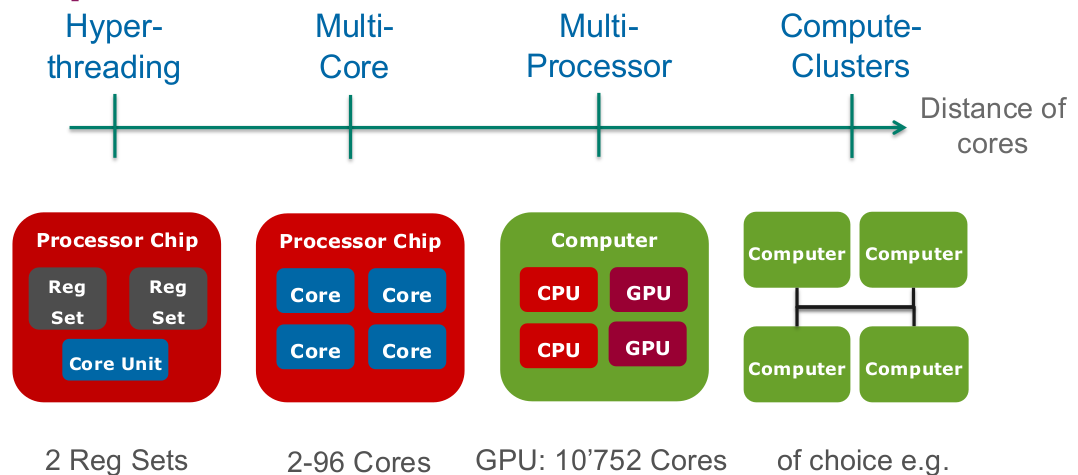
\includegraphics[width=0.7\linewidth]{res/01-levels-of-parallelism.png}

\section{Multithreading}

\begin{description}
  \item[Moores Law] \textit{(An observation)} The number of transistors within the same area (=speed of computer) will double about every two years.   Physical (atomar) limits of this law have been reached already. New ways of speeding up processors are needed.
  
  \item[Hyperthreading] Two register sets to keep two separate contexts. If one task is busy, context switch can happen fast. Two logical from one physical core. Use wait time for more efficiency. 
  Performance increase is \emph{not} 100\% the amount of logical cores.
  
  \item[Parallel] Different processors act at the same time
  
  \item[Concurrent] Time-shared, one actor. Context switches needed.
  After the end of moores law: parallelization is needed for more speedup.
  
  \item[Process] One program instance. Separate address space, high isolation. Context switches are slow, communication overhead.
  
  \item[Thread] Parallel sequence within a program / process. Each has their own stack and registers, but all threads inside a process share the same heap. Changes made are seen by other threads inside the process, heap access must be synchronized.
  
  \item[Kernel thread] Implemented in kernel, context switch with interrupt. \textit{JVM default}.
  \item[User thread] no true parallelism, just concurrency.

  \item[Thread Scheduling / Processor Multiplexing] This is concurrency: Interleaved execution. 
  Each processor can execute one thread at a time. Multiple Threads are managed via scheduling mechanisms.
  States: Running, ready, waiting.
  Context switches are "lightweight" but still have a performance impact.

  \item[synchronous] (cooperative) waiting for condition, thread queues itself as waiting
  \item[asynchronous] (preemptive) resources are released after a set amount of time
  \item[Levels of parallelism] Hyperthreading, Multi-Core, Multi-Processor, Computing-Cluster.
\end{description}
\vspace{-1mm}

\begin{minipage}[t]{0.5\linewidth}
\textbf{Interface Runnable}
\begin{lstlisting}[style=java]
class myLogic implements Runnable {
	@Override public void run() {
  }	// Thread Behavior
}
var myThr = new Thread(new myLogic());
myThr.start();
\end{lstlisting}
\end{minipage}
\begin{minipage}[t]{0.5\linewidth}
\textbf{Sub-Class of Thread}
\begin{lstlisting}[style=java]
class SimpleThread extends Thread {
	@Override public void run() {
  }	// Thread Behavior
}
var myThread = new SimpleThread();
myThread.start();
\end{lstlisting}
\end{minipage}

\begin{minipage}[t]{0.5\linewidth}
\textbf{Thread Methods}
\begin{description}
  \item[getId()] returns the identifier of the thread.
  \item[getName()] returns the name of the thread.
  \item[isAlive()] tests if the thread is alive.
\end{description}
\end{minipage}
\begin{minipage}[t]{0.5\linewidth}
  \textbf{Lambda}
  \begin{lstlisting}[style=java]
    var myThr = new Thread(() => { 
      }); // some behaviour
      myThr.start();
    \end{lstlisting}
  \end{minipage}
  \vspace{-1mm}
  
\begin{description}
  \item[getState()] returns the current state of the thread.
  \item[start()] executes the method \texttt{run()} of the thread object inside a newly created thread. If \texttt{run()} is called by the user, the runnable action will be run sequentially.
  \item[join()] \texttt{t2.join()} blocks t1 from running as long as t2 is still running. \texttt{currentThread().join()} creates a deadlock.
  \item[sleep()] running thread goes into waiting state until the time has passed for it to be ready again. Usage: \texttt{t1.sleep(ms)}
  \item[yield()] running thread releases the processor but will immediately be in ready state. Not really necessary in time-shared / preemptive scheduling. Use case: testing, low level performance (lock free data structures).
  \item[interrupt()] can be used for cooperative cancelling. What to do on an interrupt has to be defined by the programmer. 
  \item[currentThread()] get reference object to the currently running thread
  \item[setDaemon()] daemon threads are shut down when the JVM is stopped (Garbage Collector). Thread marked as daemon can be joined, making it normal again.
\end{description}

\section{Synchronization Primitives}
\textbf{Shared Ressources}: Monitor, Semaphore, Lock\&Condition, RW-Lock \\
\textbf{Timing of multiple threads:} Latch, CyclicBarrier, Semaphore

\subsection{Monitor: Mutual exclusion with Wait\&Signal Mechanism (NO FAIR)}
Every object has a lock that can be acquired using \texttt{synchronized}. Marks a \textbf{critical section} that can only be accessed by one thread at at time. Visibility is guaranteed afterwards.
\texttt{notify()}/\texttt{notifyAll()}/\texttt{wait()}: use only in synchronized block, else \texttt{IllegalMonitorStateException}.

\begin{description}
  \item[wait()] go to inner waiting room and release monitor. waits for notify.
  \item[notifyAll()] wakes all waiting threads, does not release monitor (FIFO not guaranteed)
\end{description}

Possible: \texttt{synchronized(this)}, \texttt{synchronized(this.Class)} for static method
\begin{lstlisting}[style=java]
class BankAccount {
	private int balance = 0;
	public synchronized void deposit(int amount) {
		balance += amount;
		notifyAll(); }
	public synchronized void withdraw(int amount) {
		while (balance < amount) { wait(); }
		balance -= amount; }
	public synchronized getBalance() {
		return balance; }
\end{lstlisting}
\vspace{-1mm}
\begin{minipage}[t]{0.5\linewidth}
\begin{lstlisting}[style=java]
public void method() {
	synchronized(this) {
		// code
	}
}
\end{lstlisting}
\end{minipage}
\begin{minipage}[t]{0.5\linewidth}
  \vspace{1mm}
\textbf{Issues:} always use while to \texttt{wait()}: Condition must always be checked on wakeup to ensure correctness.
Single notify(): only allowed for uniform waiting condition, when exactly 1 thread can progress.
\end{minipage}

\textbf{Pros:} powerful, object oriented \textbf{Cons:} not always optimal, inefficient with different waiting conditions, no fairness 

\subsection{Semaphor: issue free resources using counter (FAIR?)}
Is faster and more constant compared to a monitor. Can be set to fair using boolean 2nd argument. \textit{Constructor only sets initial state, can go higher than that when using release without previous acquire.}
\begin{description}
  \item[acquire()] take 1 free resource (decrement), else blocking
  \item[release()] return 1 resource (increment), notify blocked
\end{description}

\begin{lstlisting}[style=java]
class BoundedBuffer<T> {
	private Queue<T> queue = new LinkedList<>();
	private Semaphore upperLimit = new Semaphore(capacity, true);
	private Semaphore lowerLimit = new Semaphore(0, true);
	private Semaphore mutex = new Semaphore(1, true);
	public void put(T item) throws InterruptedException {
		upperLimit.acquire(); mutex.acquire(); queue.add(item); mutex.release(); lowerLimit.release(); }
	public T get() throws InterruptedException {
		lowerLimit.acquire(); mutex.acquire(); T item = queue.remove(); mutex.release(); upperLimit.release(); return item; }
\end{lstlisting}

\subsection{Lock \& Condition: Monitor with multiple waiting lists}
\textbf{Outer Wait:} Object Lock: waiting for monitor entry \\
\textbf{Inner Wait:} Condition: Wait\&Signal for multiple conditions

\begin{lstlisting}[style=java]
  class BoundedBuffer<T> {
   private Queue<T> queue = new LinkedList<>();
   private Lock monitor = new ReentrantLock(true); // fair
   private Condition nonFull  = monitor.newCondition();
   private Contition nonEmpty = monitor.newCondition();
   public void put(T item) throws InterruptedException { 
      monitor.lock(); try {
         while(queue.size() == capacity) {nonFull.await();}
         queue.add(item); nonEmpty.signal();
      }  finally { monitor.unlock(); } }
   public T get() throws InterruptedException {
      monitor.lock(); try {
         while (queue.size() == 0) { nonEmpty.await(); } 
         T item = queue.remove(); nonFull.signal(); return item;
      }  finally { monitory.unlock(); }   }  }
\end{lstlisting}

\subsection{Read-Write Locks}
Write-Lock kann nicht bezogen werden, wenn bereits ein Read Lock bezogen ist. Mehrere Read-Locks möglich.

\begin{lstlisting}[style=java]
class NameDatabase {
   private Collection<String> names = new HashSet<>() ;
   private ReadWriteLock rwLock = new ReentrantReadWriteLock(true) ; // fair
   public Collection<String> find(String pattern) { 
   rw.readLock().lock(); 
   try { for(String name : names) 
      { return name.matches(pattern) } // read only
   } finally { rwLock.readLock().unlock(); }
   public void put(String name) { 
   		rwLock.writeLock().lock(); try { names.add(name); //wr
   } finally { rwLock.writeLock().unlock(); }  }  }	
\end{lstlisting}

\subsection{Count Down Latch (x threads are waiting until counter <= 0)}
\texttt{countDown()} decrement counter, never blocks | \texttt{await()} blocks, waiting for counter <= 0 ---
Only usable once: not clear how many waiting, so latch can't be closed again.
Equal solution using Semaphores possible using release and acquire.

\begin{lstlisting}[style=java]
CountDownLatch ready = new CountDownLatch(noCars);
CountDownLatch start = new CountDownLatch(1);
carsReady.countDown(); start.await(); // car
carsReady.await(); start.countDown(); // race control
\end{lstlisting}
the same can be achieved using semaphores
\begin{lstlisting}[style=java]
var ready = new Semaphore(0); var start = new Semaphore(0);
ready.release(); start.acquire(); // car
ready.acquire(); start.release(); // race control 
\end{lstlisting}

\subsection{Cyclic Barrier (reusable barrier for fixed number of threads)}
\lstinline|await()| blocks all threads that call this function. 

\begin{lstlisting}[style=java]
CyclicBarrier raceStart = new CyclicBarrier(N); 
raceStart.await();  raceStart.getParties(); 
\end{lstlisting}

\subsection{Exchanger (Exactly two threads, blocks until other thread calls exchange(x))}
\begin{lstlisting}[style=java]
Exchanger<Integer> exchanger = new Exchanger<>(); 
for (int k = 0 ; k<2 ; k++) { new Thread(() -> {
  for (int in = 0; in < 5; in++) { 
    try { int out = exchanger.exchange(in); 
    Sysout(Thread.currentThread().getName() + 'got' + out);} 
    catch(InterruptedException) {} 
  }
}).start();}
\end{lstlisting}

\section{Dangers of Concurrency}
No synchronisation needed if objects are read only (\textit{final}, Immutability), or if an object only ever belongs to one single thread (Confinement). 

\textbf{Thread-Confinement} Object accessible via reference for one thread only \\
\textbf{Objekt-Confinement:} encaps. of inner objects by syncing all access via an outer class \\
\textbf{Thread Safety:} the avoidance of data races. \textit{When no sharing is intended}, give each thread a private copy of the relevant data.
\textit{When sharing is important}, provide explicit synchronization to make certain the program behaves in a deterministic manner.\\
\textbf{Java Collections:} newer collections are not thread safe, alternatives exist in \texttt{java.util.concurrent}

\subsection{Race Conditions (access of same resource without enough synchronization)}
Possibility of errors or undefined behaviour that should not happen according to the program logic. Knowledge of 'what is correct' is necessary to specify the error.
depends on interlocking of threads and timing of execution
\subsection{Data Race (formal error in language spec)}
two threads access the same address in memory, one of them writing, without synchronization. Data Race on volatile variables isn't possible, Race Conditions is. 

\subsection{Deadlock}
If resource graph contains a cycle. Solution: Linear order for resource locking, move locks to a higher abstraction. 
\textbf{Livelocks} block and still and use CPU cycles while waiting
\textbf{4 reasons for deadlocks}: nested locks, cyclic waiting dependencies, mutual exclusion, locking without timeout / cancelling

\subsection{Starvation (hindering of progress because of fairness problems -> Monitor)}
one thread can run the risk of having to wait 'forever' because other threads are always first to access the lock. risk when using thread priorities. Solution: fairness in synchronization.

\subsection{Correctness implies no race conditions, no deadlocks and no starvation.} 

\section{Thread Pools (Set number of available worker threads)}
Downsides of using many threads: longer wait for scheduler, start and termination, number of threads is limited, memory cost for each threads stack, full register backup at preemption.

A limited number of threads in a pool, ready to execute \textbf{independent} tasks of \textbf{potentially parallel work}. 

\subsection{Java ForkJoinPool}
Uses daemon threads, other pools have to be shut down using \texttt{myPool.shutdown()}. Tasks have to implement the \texttt{Callable} Interface.
Return values are packaged in some form (\texttt{CompletableFuture} in Java, \texttt{Task} in .NET)

\texttt{fork()} start a new task (as sub task) \\
\texttt{T join()} await task completion and get result \\
\texttt{T invoke()} start task and await result synchronously \\
\texttt{invokeAll(t1, t2)} start several tasks and await results \\
\texttt{execute()} arrange async execution \\
\texttt{submit()} arrange execution and obtain future

\begin{lstlisting}[style=java]
var threadPool = new ForkJoinPool(); // custom pool
var pool = ForkJoinPool.commonPool(); // default,singleton
Future<Integer> future = threadPool.submit(() -> {
    int value = ...; // long calculation
    return value;  });
int result = future.get(); // blocking call
\end{lstlisting}
\textbf{Recursive Action Example}
\begin{lstlisting}[style=java]
class PairwiseSum extends RecursiveAction {
  private final int[] array;
  private final int lower, upper;
  private static final int THRESHOLD = 1; // configurable
  public PairwiseSum(int[] array, int lower, int upper) {
    this.array = array; this.lower = lower; this.upper = upper; }
  @Override protected void compute() {
    if (upper - lower > THRESHOLD) {
      int middle = (lower + upper) / 2;
      invokeAll(
        new PairwiseSum(array, lower, middle),
        new PairwiseSum(array, middle, upper)
      );
    } else {
      for (int i = lower; i < upper; i++) {
        array[2 * i] += array[2 * i + 1];
        array[2 * i + 1] = 0;
      }  }  }  }
\end{lstlisting}

\subsection{.NET Task Parallel Library}
Multiple abstraction layers: \textit{Task Parallelization} uses tasks explicitly, \textit{Data Parallelization} uses parallel statements and queries (implicit tasks) and \textit{Asynchronous Programming (async/await)}

\textbf{Exception in threads} terminate the program.
\textbf{Fairness flag} not available.
\textbf{Lock\&Condition} not available.
\textbf{ReadWriteLockSlim} for upgradeable Read/Write Lock.
\textbf{Semaphores} can be used at OS level.
\textbf{Mutex} binary semaphore at OS level
\textbf{Collections} are not thread safe, except \texttt{System.Collections.Concurrent}

\begin{lstlisting}[style=java]
  Task task = Task.Run(() => {
    // task implementation
  }); // other code
  task.Wait(); // blocking, without return value
  Console.Write(task.Result); // blocking, get result
\end{lstlisting}

Nested tasks are possible:
\begin{lstlisting}[style=java]
  var task = Task.Run(() => {
    var left = Task.Run(() => Count(leftPart));
    var right = Task.Run(() => Count(rightPart));
    return left.Result + right.Result;
  });
\end{lstlisting}

\begin{minipage}[t]{0.5\linewidth}
  Implicit Tasks, wait barrier at the end: 
  \begin{lstlisting}[style=java]
  Parallel.Invoke(
    () => MergeSort(l, m),
    () => MergeSort(m, r)
  );
  \end{lstlisting}
\end{minipage}
\begin{minipage}[t]{0.5\linewidth}
  Data Parallel for each:
  \begin{lstlisting}[style=java]
  Parallel.ForEach(list, 
    file => Convert(file)
  );
  \end{lstlisting}
\end{minipage}

Data Parallel for (when iterations are independent):
\begin{lstlisting}[style=java]
  Parallel.For(0, array.Length, 
    i => DoComputation(array[i])
  );
\end{lstlisting}

Parallel Loops will automatically group multiple iterations into one single task to avoid too much overhead.

\subsection{.NET Parallel LINQ}

\begin{lstlisting}[style=java]
  from book in bookCollection.AsParallel().AsOrdered()
    where book.Title.Contains("Concurrency")
    select book.ISBN
\end{lstlisting}

\section{Asynchronous Programming}

\begin{lstlisting}[style=Java]
CompletableFuture<Long> fut = CompletableFuture.supplyAsync(() -> {
	longOp(); });
fut.thenAccpet(res -> System.out.println(res));
\end{lstlisting}
\vspace{1mm}
\begin{lstlisting}[style=Java]
// Wait for all Futures
CompletableFuture.allOf(fut1, fut2).thenAccept(cont);
//Wait for ANY Future to arrive
CompletableFuture.any(fut1, fut2).thenAccept(cont);
\end{lstlisting}

\section{Memory Models (Lock free data structures = efficient synchronization)}
\textbf{Volatile:} no data race possible. changes are immediately visible for other threads. no statement reordering by compiler. atomic read/write even for long/double \\
\textbf{Atomicity:} read/write Access of variables is by default atomic for: primitive types up to 32 bit, objet references. \\
\textbf{Visibility:} changes to a variable are not immediately visible to other threads.

Visibility is guaranteed by
\begin{itemize}
	\item Locks (changes before release are visible when acquiring)
	\item Volatile variable (change visible immediately)
	\item final variables when initialized (after end of constructor) (but it's a no no)
	\item threat start/join, task start/end
\end{itemize}

\textbf{Volatile Visibility}: All previous changes to a volatile variable become visible when it is accessed. Read/write access invalidates the main memory (Memory Flush).

\subsection{.NET Memory Model (Differences to Java)}
\begin{itemize}
	\item Atomicity: long/double not atomic with volatile
	\item Visibility: not defined. implicit with order.
	\item Ordering: volatile ist nur partielle fence
	\item Atomic instructions using class \texttt{Interlocked}
\end{itemize}

\subsection{Java: Atomic Objects (No blocking or waiting for locks. Yes ordering and visibility)}

\begin{lstlisting}[style=java]
AtomicReference<Object>; AtomicInteger(); AtomicBoolean();
\end{lstlisting}
Objects provide methods for atomic operations, usually returns the previous value.
\vspace{-1mm}

\texttt{updateAndGet(), getAndUpdate(), addAndGet(x), getAndAdd(x), compareAndSet(old, new)}

\textbf{Optimistische Synchronisation}
\begin{lstlisting}[style=java]
do { oldValue = var.get(); newValue = calculateChanges(oldValue);
} while (!var.compareAndSet(oldValue, newValue);
\end{lstlisting}

\textbf{Java Lock-Free Data Structures} \\
Verwenden den \textit{compare and set} Algorithmus und verwendet keine Locks. \\
\texttt{ConcurrentLinkedList<>();}
\texttt{ConcurrentHashMap<K, V>();}

\begin{lstlisting}[style=java]
while (true) {
  var current = top.get();
  var node = new Node<>(value, current);
  if (top.compareAndSet(current, node)) { return; } 
  else { Thread.yield(); } }
\end{lstlisting}
\vspace{1mm}
\begin{lstlisting}[style=java]
top.updateAndGet(current -> new Node<>(value, current));
\end{lstlisting}

\section{.NET Interlocked}
\begin{lstlisting}[style=java]
Interlocked.Add(val1, val2)
Interlocked.Increment(val1), Interlocked.Decrement(val1)
Interlocked.CompareExchange(val1, val2, val3) // compare first two, if equal exchange 1 with 3
Interlocked.Exchange(val1, val2) // Sets val1 to val2 and returns the original value
Interlocked.MemoryBarrier() // no reordering across here
\end{lstlisting}

\section{Examples}
\textbf{Blocking Queue mit Non Blocking Datenstrukturen}
\begin{lstlisting}[style=csharp]
public class BlockingQueue<T>{
	private final Semaphore capacity;
	private final Queue<T> qu = new ConcurrentLinkedList<>();
	private final Semaphore size = new Semaphore(0);
	public BlockingQueue(int capacity){
		this.capacity = new Semaphore(capacity);
	}
	public void add(T item) throws InterrruptedException{
		capacity.aquire(); qu.add(item); size.release();
	}
	public T remove() throws InterrruptedException{
		size.aquire(); var item = qu.remove(); capacity.release();
		return item;
}}
\end{lstlisting}


\textbf{Java Thread Pool}
\begin{lstlisting}[style=java]
public class ThreadPool {
  private final int poolSize;
  private final BlockingQueue<Runnable> taskQueue;
  private final ThreadPoolExecutor executor;
  public ThreadPool(int size) {
    this.poolSize = size;
    this.taskQueue = new LinkedBlockingQueue<>();
    this.executor = new ThreadPoolExecutor(poolSize, poolSize, 0L, TimeUnit.MILLISECONDS, taskQueue);
  }
  public void submit(Runnable task) {
    executor.execute(task); } }
\end{lstlisting}

\textbf{Rekursive Höhekalkulierung}
\begin{lstlisting}[style=java]
int height = threadPool.invoke(new HeightCalculation(tree));
// task implemenation
class HeightCalculation extends RecursiveTask<Integer> {
  private final Node node;

  public HeightCalculation(Node node) { this.node = node; }
  
  @Override protected Integer compute() {
    if (node == null) { return 0; }
    var lt = new HeightCalculation(node.getLeft()); 
    var rt = new HeightCalculation(node.getRight()); 
    lt.fork(); rt.fork();
    return Math.max(rt.join(), lt.join()) + 1;
  } 
}
\end{lstlisting}

\textbf{Task Graph Traversal}
\begin{lstlisting}[style=csharp]
Thread Pool: Tree Traversal
class TreeTraversal extends RecursiveAction {
  private final Node node;
  public TreeTraversal(Node node) { this.node = node; }
  
  @Override
  protected void compute() {
    if (node != null) {
      TreeTraversal lt = new TreeTraversal(node.getLeft());
      TreeTraversal rt = new TreeTraversal(node.getRight());
      lt.fork(); rt.fork(); 
      Logic.operation(node.getValue());
      rt.join(); lt.join(); } } }
\end{lstlisting}